\chapter{Mechanics}

\section{Overview}

\paragraph{} OpenCombat is a free and open-source 2D platform fighting game where players punch, kick, grab, block, dodge and use their super powers to knock out all their opponents in intense and fast-paced battles across diverse arenas. Players can embrace the chaos by fighting 4v4 free-for-alls with items \textit{(generously provided by the audience)} or show off their skills in competitive 1v1 matches; the rules are completely customizable in both offline and online play. Players can also create their own combatants and choose from 1 of 4 different classes each with their own unique set of moves. By completing objectives and playing matches, players will earn badges that they can proudly display on their profile.

\paragraph{} At the core of OpenCombat is the players and their experiences inside and outside the game. OpenCombat is free and all subsequent updates will also be free requiring no monthly subscriptions or purchases to acquire new content. Since the game is open source, players can create plugins or take part in helping to add new features, fix bugs or balance gameplay. One of the essential experiences of fighting games is coming together with others and playing multiplayer locally; players can use the in-game community organizing tool to host or attend events in their area.

\section{Combat}

\subsection{Overview}

\paragraph{} Similarly to other platform fighting games, OpenCombat matches are fought on stages with varying platform layouts between 2 to 4 players. Players coming from the previously mentioned games will be familiar with the simple button-and-direction execution of actions. These actions include:

\begin{itemize}
    \item Neutral attack, throw item (A with or without direction).
    \item Special attack (B with or without direction).
    \item Strong attack (X with or without direction).
    \item Jump (Y).
    \item Block (L2 or R2 without direction).
    \item Dodge (L2 or R2 with direction).
    \item Grab (L1 or R1).
    \item Taunt (D-Pad).
\end{itemize}

\paragraph{} The OpenCombat experience distinguishes itself from these titles by including new actions and mechanics from 2D traditional fighting games such as:

\begin{itemize}
    \item Stocks and percent are replaced with rounds, matches and stamina from traditional fighting games.
    \item Specials and strong attacks, like neutral attacks, have an aerial variation.
    \item Knockback and stun are significantly reduced and do not scale with damage.
\end{itemize}

\paragraph{} Players will utilize all of these actions in order to be the last one remaining. Players can block incoming players' attacks, grab their blocking opponents to catch them off-guard or seize the opportunity to strike if they try to grab them. Players can also take advantage of the unique platform layouts of each stage to put themselves in a position to take the upper hand. Players are eliminated when their stamina reaches 0 or they have been knocked out of the ring.

\paragraph{} The players have complete control over the rules they choose to play with whether they are playing offline or online. Some of these options include:

\begin{itemize}
    \item Rounds
    \item Stamina
    \item Items
    \item Teams
    \item Physics
\end{itemize}

\subsection{Items}

\paragraph{} The audience of a match can throw items into the arena for combatants to use. The audience is usually tame and only throws items into the ring if they have a reason.

\subsubsection{Concessions}

\paragraph{} If the combatants bore the audience by not attacking each other for a while, they will start throwing their trash into the arena. Clever combatants can pick up the ones that don't explode and throw them at their opponents for light amounts of damage.

\subsubsection{Underwear}

\paragraph{} When one of the combatants successfully pulls off a taunt, some of the more zealous fans in the audience will throw their boxers, bras, briefs and panties into the arena. Combatants have to be careful though because the smell of the underwear can cause small incremental damage to those close by. Underwear can be thrown but they have little to no momentum.

\subsubsection{Confetti F-Bombs}

\paragraph{} When one of the combatants in a match with 3 or more is eliminated, the audience pays their respects by throwing confetti bombs shaped like the letter F into the arena. Combatants can try to catch them as they fall but if they fail to do so, they explode on impact for massive damage.

\subsubsection{Headphones}

\paragraph{} When a Berserker is getting beaten badly, a pair of headphones is thrown into the arena that, when picked up, play an enraging voice line. The combatant who heard it gets a temporary strength and speed boost.

\paragraph{} Some of the voice lines that will be played include the following:

\begin{itemize}
    \item It's pronounced "jif."
    \item Your favorite anime is trash.
    \item Pineapple doesn't belong on pizza.
    \item Always put the ketchup on top of your fries.
    \item Pour the milk in the bowl before you add the cereal.
    \item Water is not wet.
    \item Hot dogs are sandwiches.
    \item You want to listen to my mixtape?
    \item I brush my teeth without wetting the bristles.
\end{itemize}

\subsubsection{Tome}

\paragraph{} Concerned that their favorite mage combatant is losing, the audience will start throwing in tomes to help them out. Since combatants don't have time to study the text, they can use it as a heavy projectile to toss at opponents.

\subsubsection{Ale}

\paragraph{} When a sailor is losing in combat, the audience will start tossing ale into the arena to help them out. Drinking the ale will slow down the player's attacks but make them more powerful; they can also toss the empty bottle at opponents for moderate damage.

\subsubsection{Treats}

\paragraph{} The allies of druids will toss animal treats into the arena if the Druid is losing. When consumed, these treats restore a little health and the empty bag can be tossed at opponents for light damage.

\subsubsection{Battleaxe}

\paragraph{} To the shock of many, someone in the audience was allowed to bring in a battleaxe and tosses it into the arena when heavies are losing. Only large fighters can pick up the axe and although it does not move quickly or go far when thrown, it deals a lot of damage on impact.

\subsubsection{Zen Grass}

\paragraph{} The audience will toss in a jar of zen grass if their favorite monk is being beaten. Regardless of who picks this up, everyone is slowed down temporarily.

\section{Matchmaking, Player Profiles and the Community Organizing Tool}

\paragraph{} Players can fight it out online in private matches or by using online matchmatching. When players first start the game, they create a local profile that is used to keep track of their wins, losses and other in-game data. These profiles can be synced to an optional online account so players can simply log in and have access to their information from anywhere. At any point, the player can choose to reset their progress and have their data deleted.

\paragraph{} The community organizing tool is designed for every type of user from the college sophomore looking to have some friends over to the tournament organizer preparing for a large event. Organizers can post information about their event, track attendance, setup brackets and quickly communicate with all parties involved to coordinate without needing social media or external services. The average player will find the community organizing tool to be a helpful way to plan ahead for social gatherings as well as find local events to play at. To encourage players to come together and plan community events, player profiles will have a community level where experience is gained from playing matches at community events, hosting events and being commended by your fellow players for sportsmanship, teamwork, positivity, etc.

\section{Custom Combatants}

\paragraph{} Players can create their own custom combatant based on 1 of 4 classes. They can customize their physical appearance, clothing and biographical information. Each of these classes come with their own movesets, strengths and weaknesses.

\subsection{Playable Classes}

\subsubsection{Mage}

\begin{description}
    \item[Archetype] Zoner
    \item[Body Size] Medium
\end{description}

\paragraph{Description} Combatants who can wield the arcane arts use it to control the space around them and keep their opponents away. Although these fighters move on the ground at a moderate speed, they are able to better control their aerial movement despite their average weight. While they are great at keeping slower opponents away, they are weak against opponents that can rush and attack them.

\subsubsection{Sailor}

\begin{description}
    \item[Archetype] Grappler
    \item[Body Size] Medium
\end{description}

\paragraph{Description} From the sea to the shore, sailors are the undisputed masters of the cutlass and hookshot. Their average mobility, power and speed are offset by their ability to pull distant opponents towards them. The sailors' hookshots give them a distinct advantage over range opponents but they can be easily be overwhelmed by faster fighters.

\subsubsection{Berserker}

\begin{description}
    \item[Archetype] Rushdown
    \item[Body Size] Small
\end{description}

\paragraph{Description} Wielding small axes and a thirst for blood, Berserkers are able to harnass their rage to overwhelm their foes. They are the quickest combatants on the ground and are able to rush into combat easily. This makes them adept at navigating around projectiles to smother distance-based opponents, however, they have difficulty with large or armored opponents.

\subsubsection{Monk}

\begin{description}
    \item[Archetype] Aerial
    \item[Body Size] Small
\end{description}

\paragraph{Description} Using paragliders and karate, these combatants maneuver smoothly in the air and fight from the skies. Their extremely light weight helps them escape combos easier but their ground combat skills and grappling leave much to be desired. They excel against large and slow opponents but can easily be overwhelmed by ranged attacks or easily smothered by fast fighters.

\subsubsection{Druid}

\begin{description}
    \item[Archetype] Grappler
    \item[Body Size] Large
\end{description}

\paragraph{Description} The combatants most in-tune with nature leverage its power to transform parts of their body into various flora and fauna. Whether it is grabbing their opponents with talons or protecting themselves with tree bark, these combatants are renowned for their ingenuity in combat. Although they can smother smaller opponents with their strength, ranged and aerial opponents can easily outmaneuver them.

\subsubsection{Heavy}

\begin{description}
    \item[Archetype] Rushdown
    \item[Body Size] Large
\end{description}

\paragraph{Description} Equipped with the largest armor and weaponry they could find, these combatants pride themselves on their ability to withstand damage. Their speed is the slowest of all the combatants but they also do the most damage with their massive strikes. Their lack of dexterity leaves them vulnerable to grappling opponents but their armor makes them resilient against small and fast foes.

\subsection{Races and Body Sizes}

\begin{table}[h!]
    \centering
    \begin{tabular}{c|c|c}
    Small  & Medium & Large   \\
    \hline
    Gnome  & Human  & Kong    \\
    Dwarf  & Elf    & Troll   \\
    Goblin & Orc    & Goliath \\
    Corgo  & Purr   & Drake  
    \end{tabular}
\end{table}

\section{Flow}

\subsection{Match}

\paragraph{} Players who want to play a match start by choosing which rules they want to use. From there, they pick the stage first so another player cannot intentionally pick a stage their opponent's character is weaker on. Players will then select which character they want to use and start the match. Combat will largely consist of players blocking, dodging and attempting to find openings to exploit. If only one player remains with more than 0 HP or only one player did not get knocked out of the arena, they win the round. This will repeat until a player has won the majority of rounds. After that, players can change any of their previous selections, rematch or quit.

\begin{figure}[h!]
    \centering
    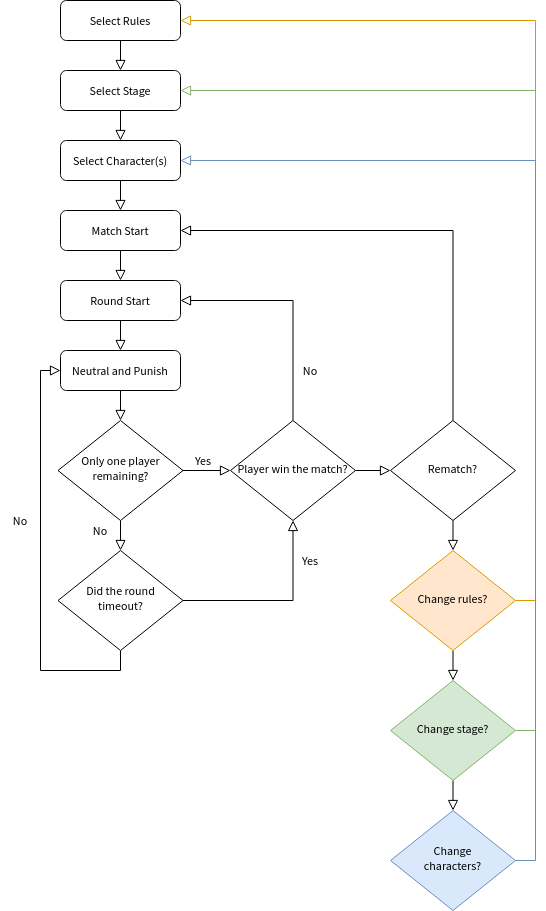
\includegraphics[width=0.5\linewidth]{images/flow-match.png}
    \caption{The flow of the match from choosing the rules to choosing what happens when the set ends.}
\end{figure}

\subsection{State Machine}

\paragraph{} The game follows a simple state machine that is similar to other games. From the main menu, players can access the default play mode, the customization tools, the community organizing tool and basic settings. In the customization menu (referred to as the Locker Room), players can change their controls and customize their characters. In the community organizing tool, players can plan events, attend other peoples' events, manage their profiles and learn about news related to the game as well as the community. The settings menu allows players to adjust the basic aspects of the experience like audio levels, graphical quality and subtitles.

\begin{figure}[h!]
    \centering
    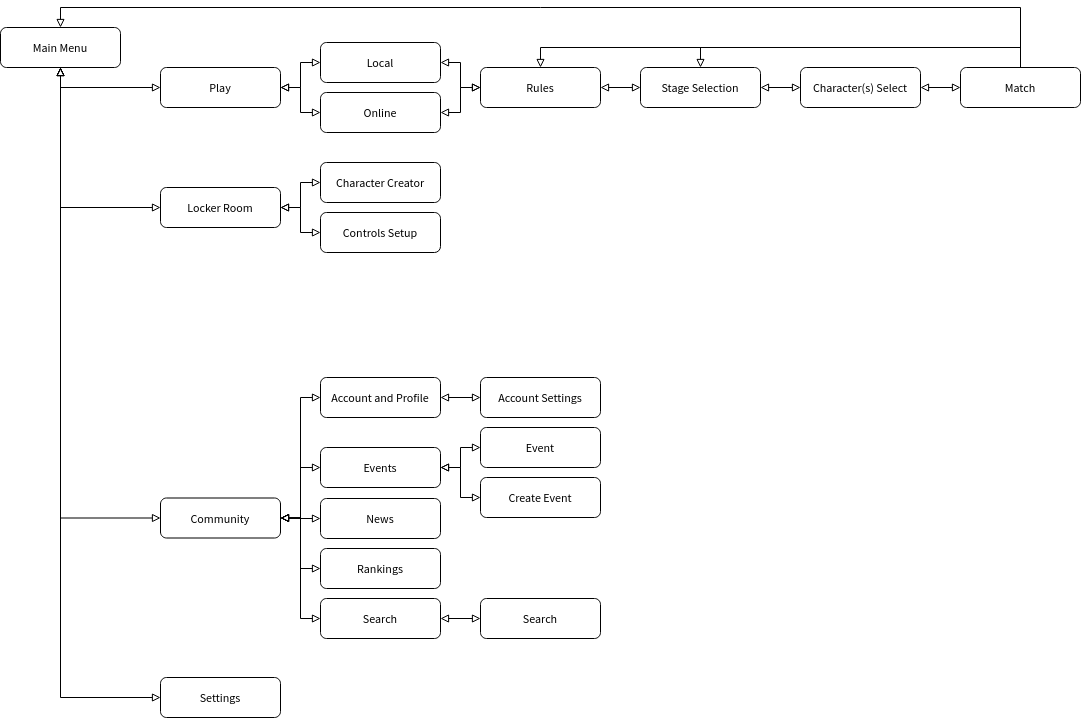
\includegraphics[width=0.75\linewidth]{images/flow-menu.png}
    \caption{The flow of the state machine and how players can navigate the menus.}
\end{figure}